%%%%%%%%%%%%%%%%%%%%%%%%%%%%%%%%%%%%
% Slide options
%%%%%%%%%%%%%%%%%%%%%%%%%%%%%%%%%%%%

% Option 1: Slides with solutions

\documentclass[slidestop,compress,mathserif]{beamer}
\newcommand{\soln}[1]{\textit{#1}}
\newcommand{\solnGr}[1]{#1}

% Option 2: Handouts without solutions

%\documentclass[11pt,containsverbatim,handout]{beamer}
%\usepackage{pgfpages}
%\pgfpagesuselayout{4 on 1}[letterpaper,landscape,border shrink=5mm]
%\newcommand{\soln}[1]{ }
%\newcommand{\solnGr}{ }


%%%%%%%%%%%%%%%%%%%%%%%%%%%%%%%%%%%%
% Style
%%%%%%%%%%%%%%%%%%%%%%%%%%%%%%%%%%%%

\def\chp3@path{../../Chp 3}
\input{../../lec_style.tex}


%%%%%%%%%%%%%%%%%%%%%%%%%%%%%%%%%%%%
% Preamble
%%%%%%%%%%%%%%%%%%%%%%%%%%%%%%%%%%%%

\title[Lecture 8]{MA213: Lecture 8}
\subtitle{Module 2: Probability, Random Variables, and Distributions}
\author{OpenIntro Statistics, 4th Edition}
\institute{$\:$ \\ {\footnotesize Based on slides developed by Mine \c{C}etinkaya-Rundel of OpenIntro. \\
The slides may be copied, edited, and/or shared via the \webLink{http://creativecommons.org/licenses/by-sa/3.0/us/}{CC BY-SA license.} \\
Some images may be included under fair use guidelines (educational purposes).}}
\date{}

%%%%%%%%%%%%%%%%%%%%%%%%%%%%%%%%%%%%
% Begin document
%%%%%%%%%%%%%%%%%%%%%%%%%%%%%%%%%%%%

\begin{document}


%%%%%%%%%%%%%%%%%%%%%%%%%%%%%%%%%%%%
% Title page
%%%%%%%%%%%%%%%%%%%%%%%%%%%%%%%%%%%%

{
\addtocounter{framenumber}{-1} 
{\removepagenumbers 
\usebackgroundtemplate{\includegraphics[width=\paperwidth]{../../OpenIntro_Grid_4_3-01.jpg}}
\begin{frame}

\hfill \includegraphics[width=20mm]{../../oiLogo_highres}

\titlepage

\end{frame}
}
}


%%%%%%%%%%%%%%%%%%%%%%%%%%%%%%%%%%%%
% Recap/Agenda 
%%%%%%%%%%%%%%%%%%%%%%%%%%%%%%%%%%%%
% TODO better formatting
\begin{frame}
    \frametitle{Module 2: Probability, Random Variables, and Distributions}
    \begin{itemize}
        \item \hl{Previously: } Conditional Probability, Sampling (Chapters 3.2-3.3)
        \item \hl{This time: } Random Variables (Chapter 3.4)
        \item \hl{Reading: } Chapter 3.5 for next time
        \item \hl{Deadlines/Announcements: } 
        \begin{itemize}
            \item Quiz 1 in discussions next week
            \item HW 3 due Monday
        \end{itemize}
    \end{itemize}
    
\end{frame}

%%%%%%%%%%%%%%%%%%%%%%%%%%%%%%%%%%%%
% Learning objectives:
%%%%%%%%%%%%%%%%%%%%%%%%%%%%%%%%%%%%
\begin{frame}
    \frametitle{Learning Objectives}
    \begin{itemize}
        \item \textbf{M2, LO1: Validate and Explain Probability Distributions:} Assess the validity of a probability distribution using the concepts of outcome, sample space, and probability properties (e.g., disjoint outcomes, probabilities between 0 and 1, and total probabilities summing to 1).
        \item \textbf{M2, LO3: Compute Probabilities Using Various Tools:} Use logic, Venn diagrams, and probability rules to compute probabilities for events.
        \item \textbf{M2, LO4: Understand and Compute Expectations and Variances:} Explain the concepts of expectations and variances of random variables, and compute the expectation and variance of a linear combination of random variables.
    \end{itemize}
\end{frame}


%%%%%%%%%%%%%%%%%%%%%%%%%%%%%%%%%%%%
% Sections
%%%%%%%%%%%%%%%%%%%%%%%%%%%%%%%%%%%%

\subsection{Tree diagrams}

%%%%%%%%%%%%%%%%%%%%%%%%%%%%%%%%%%%%

\begin{frame}
\frametitle{Inverting probabilities}

\dq{When a patient goes through breast cancer screening there are two competing claims: patient had cancer and patient doesn't have cancer. If a mammogram yields a positive result, what is the probability that patient actually has cancer?}

\twocol{0.7}{0.3}{
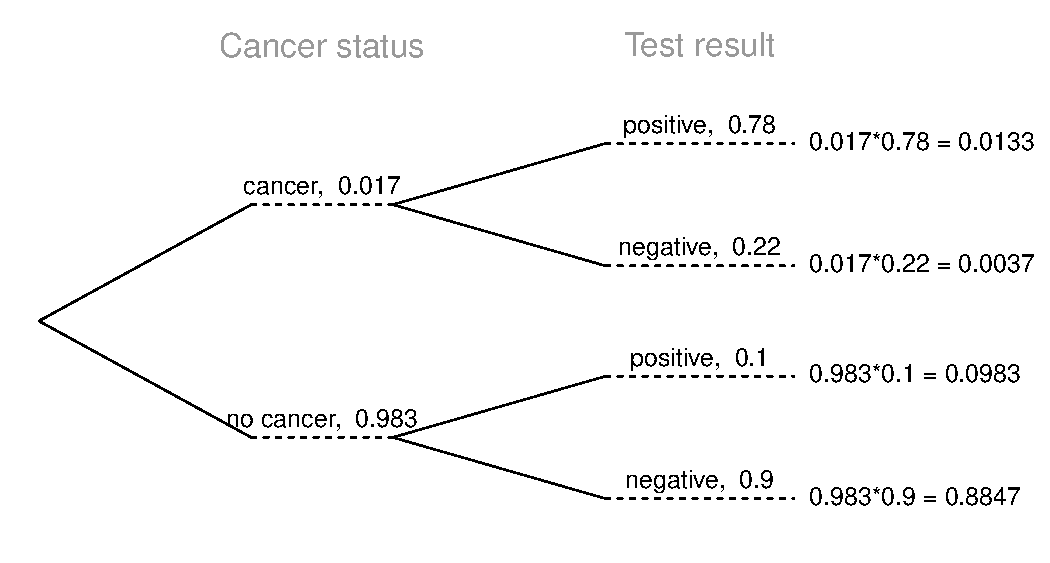
\includegraphics[width=\textwidth]{\chp3@path/3-2_conditional_probability/figures/cancer_tree/cancer_tree_first} 
}
{
\pause
{\footnotesize
\begin{eqnarray*}
&&P(C | +) \\
\pause
&&= \frac{P(C~and~+)}{P(+)} \\
\pause
&&= \frac{0.0133}{0.0133 + 0.0983} \\
\pause
&&= 0.12
\end{eqnarray*}
}
}

\pause

\Note{Tree diagrams are useful for inverting probabilities: we are given $P(+|C)$ and asked for $P(C|+)$.}

\end{frame}

%%%%%%%%%%%%%%%%%%%%%%%%%%%%%%%%%%%

\subsection{Bayes' Theorem}

%%%%%%%%%%%%%%%%%%%%%%%%%%%%%%%%%%%%

\begin{frame}
\frametitle{Bayes' Theorem: Version 1}

The conditional probability formula we have seen so far is a special case of \hl{Bayes' Theorem}, which lets us switch the conditioning.

\vspace{2mm}
\[
P(B|A) = \frac{P(A \cap B)}{P(A)} \implies P(A \cap B) = P(B|A)P(A)
\]
\pause
\[
P(A|B) = \frac{P(A \cap B)}{P(B)} = \frac{P(B|A)P(A)}{P(B)}
\]

\pause
\vspace{2mm}

\formula{Bayes' Theorem (1):}{
\[
P(A|B) = \frac{P(B|A)P(A)}{P(B)}
\]
}

\end{frame}

% --- Bayes' Theorem Step 2 ---
\begin{frame}
\frametitle{Bayes' Theorem: Version 2}
We often don't know the marginal probability $P(B)$ by itself, so we split the denominator:
\formula{Bayes' Theorem (2):}{
\[
P(A|B) = \frac{P(B|A)P(A)}{P(B)} = \frac{P(B|A)P(A)}{P(B|A)P(A) + P(B|A^c)P(A^c)}
\]
}

\pause
\vspace{2mm}

\begin{center}
	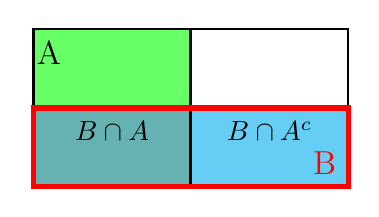
\begin{tikzpicture}[scale=1.0]
		% Draw the main rectangle (sample space)
		\draw[thick] (0,0) rectangle (4,2);

		% (right half, bottom)
		\fill[cyan!60] (2,0) rectangle (4,1);

		% (top left)
		\fill[green!60] (0,1) rectangle (2,2);

		% (bottom left)
		\fill[teal!60] (0,0) rectangle (2,1);

		% Labels
		\node[red] at (3.7,0.3) {\large B};
		\node at (0.2,1.7) {\large A};
		\node at (3,0.7) { $B \cap A^c$};
		\node at (1,0.7) { $B \cap A$}; 

		% Draw A and B outlines
		\draw[thick, black, line width=1pt] (0,0) rectangle (2,2);
		\draw[thick, red, line width=2pt] (0,0) rectangle (4,1);
	\end{tikzpicture}
\end{center}
\pause
\small{Note: $P(B \cap A)=P(B|A)P(A)$ and $P(B \cap A^c)=P(B|A^c)P(A^c)$, by the conditional probability formula (again!)}


\end{frame}

% --- Bayes' Theorem Step 3 ---
\begin{frame}
\frametitle{Bayes' Theorem: Version 3}


This trick can be extended to more than two mutually exclusive events $A_1, A_2, \ldots, A_k$ that \hl{partition} the sample space.

\formula{Bayes' Theorem (3):}{
\[ P(A_1|B) = \frac{P(B|A_1)P(A_1)}{P(B|A_1)P(A_1) + P(B|A_2)P(A_2) + \cdots + P(B|A_k)P(A_k)} \]
\[ = \frac{P(B|A_1)P(A_1)}{\sum_{i=1}^k P(B|A_i)P(A_i)}\]
}
\pause

\begin{center}
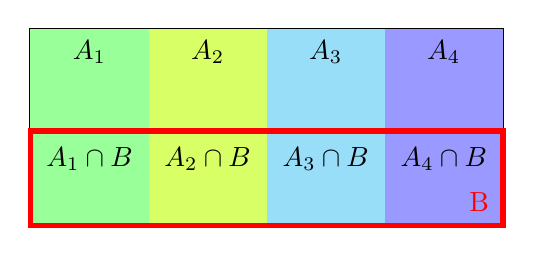
\begin{tikzpicture}[scale=1.0]
	% Draw universal set
	\draw[thick] (0,0) rectangle (6,2.5);
	% Draw A1, A2, A3, A4
	\foreach \i/\col in {1/green!40,2/lime!60,3/cyan!40,4/blue!40} {
		\fill[\col] (1.5*\i-1.5,0.0) rectangle (1.5*\i,2.5);
		\node at (-0.75+1.5*\i,2.2) {$A_{\i}$};
	}
	% Draw B as a horizontal bar
	\draw[thick,red, line width=2pt] (0,0.0) rectangle (6,1.2);
	% Label intersections
	\foreach \i in {1,2,3,4} {
		\node at (-0.75+1.5*\i,0.85) {$A_{\i} \cap B$};
	}
	% Label B
	\node[red] at (5.7,0.3) {B};
\end{tikzpicture}
\end{center}

\end{frame}

%%%%%%%%%%%%%%%%%%%%%%%%%%%%%%%%%%%%
\begin{frame}
\frametitle{Law of Total Probability}
The trick we used in the denominator of Bayes' Theorem is called the \hl{Law of Total Probability}.

\vspace{1em}
\formula{Law of Total Probability}{
\[ P(B) = P(B|A_1)P(A_1) + P(B|A_2)P(A_2) + \cdots + P(B|A_k)P(A_k) \]
\[ P(B) = \sum_{i=1}^k P(B|A_i)P(A_i) \]
} 

\vspace{1em}
\begin{itemize}
  \item The events $A_1, A_2, \ldots, A_k$ must be mutually exclusive and exhaustive (i.e. partition the sample space).
  \item We are computing the \hl{marginal probability} of $B$ by \hl{marginalizing} over the $A_i$'s.
\end{itemize}
\end{frame}

%%%%%%%%%%%%%%%%%%%%%%%%%%%%%%%%%%%%%
\begin{frame}
\frametitle{Bayes' Theorem Example: Weather Prediction}

\begin{itemize}
	\item Let $A_1$ = \{rain tomorrow\}, $A_2$ = \{cloudy tomorrow\}, $A_3$ = \{clear tomorrow\}, $B$ = \{weatherman predicts rain\}.
	\item Assume $P(A_1) = 0.2$, $P(A_2) = 0.15$, $P(A_3) = 0.65$
	\item $P(B|A_1) = 0.8$, $P(B|A_2) = 0.4$, $P(B|A_3) = 0.2$
	\item What is $P(A_1|B)$?
\end{itemize}

\vspace{2mm}
\pause
\[
P(A_1|B) = \frac{P(A_1)P(B|A_1)}{P(A_1)P(B|A_1) + P(A_2)P(B|A_2) + P(A_3)P(B|A_3)}
\]

\begin{align*}
P(A_1|B) &= \frac{0.2 \times 0.8}{0.2 \times 0.8 + 0.15 \times 0.4 + 0.65 \times 0.2} \\
				&= \frac{0.16}{0.16 + 0.06 + 0.13} \\
				&= \frac{0.16}{0.35} \\
				&= 0.46
\end{align*}
\end{frame}


%%%%%%%%%%%%%%%%%%%%%%%%%%%%%%%%%%%
\section{Edfinity Quiz}
%%%%%%%%%%%%%%%%%%%%%%%%%%%%%%%%%%%


%%%%%%%%%%%%%%%%%%%%%%%%%%%%%%%%%%%%

\section{Sampling from a small population}

%%%%%%%%%%%%%%%%%%%%%%%%%%%%%%%%%%%%

\begin{frame}
\frametitle{Sampling with replacement}

When sampling \hl{with replacement}, you put back what you just drew.

\pause

\begin{itemize}

\item Imagine you have a bag with 5 red, 3 blue and 2 orange chips in it. What is the probability that the first chip you draw is blue?
\begin{center}
5 \textcolor{red}{$\CIRCLE$}~, 3 \textcolor{blue}{$\CIRCLE$}~, 2 \textcolor{orange}{$\CIRCLE$}
\end{center}

\pause

\[ Prob(B_1) = \frac{3}{5 + 3 + 2} = \frac{3}{10} = 0.3 \]

\pause

\item Suppose you did indeed pull a blue chip in the first draw. If drawing with replacement, what is the probability of drawing a blue chip in the second draw?

\pause

\begin{center}
$1^{st}$ draw: 5 \textcolor{red}{$\CIRCLE$}~, 3 \textcolor{blue}{$\CIRCLE$}~, 2 \textcolor{orange}{$\CIRCLE$} \\

\pause

$2^{nd}$ draw: 5 \textcolor{red}{$\CIRCLE$}~, 3 \textcolor{blue}{$\CIRCLE$}~, 2 \textcolor{orange}{$\CIRCLE$}
\end{center}

\pause

\[ Prob(B_2 | B_1) = \frac{3}{10} = 0.3 \]

\end{itemize}

\end{frame}

%%%%%%%%%%%%%%%%%%%%%%%%%%%%%%%%%%%%%

\begin{frame}
\frametitle{Sampling with replacement (cont.)}

\begin{itemize}

\item Suppose you actually pulled an orange chip in the first draw. If drawing with replacement, what is the probability of drawing a blue chip in the second draw?

\pause

\begin{center}
$1^{st}$ draw: 5 \textcolor{red}{$\CIRCLE$}~, 3 \textcolor{blue}{$\CIRCLE$}~, 2 \textcolor{orange}{$\CIRCLE$} \\
\pause
$2^{nd}$ draw: 5 \textcolor{red}{$\CIRCLE$}~, 3 \textcolor{blue}{$\CIRCLE$}~, 2 \textcolor{orange}{$\CIRCLE$}
\end{center}
\pause
\[ Prob(B_2 | O_1) = \frac{3}{10} = 0.3 \]

\pause
\item If drawing with replacement, what is the probability of drawing two blue chips in a row?
\begin{center}

\pause
$1^{st}$ draw: 5 \textcolor{red}{$\CIRCLE$}~, 3 \textcolor{blue}{$\CIRCLE$}~, 2 \textcolor{orange}{$\CIRCLE$} \\
$2^{nd}$ draw: 5 \textcolor{red}{$\CIRCLE$}~, 3 \textcolor{blue}{$\CIRCLE$}~, 2 \textcolor{orange}{$\CIRCLE$}
\end{center}
\pause
\[ Prob(B_1) \cdot Prob(B_2 | B_1) = 0.3 \times 0.3 \]
\[ = 0.3^2 = 0.09 \]

\end{itemize}

\end{frame}

%%%%%%%%%%%%%%%%%%%%%%%%%%%%%%%%%%%%%

\begin{frame}
\frametitle{Sampling with replacement (cont.)}

\begin{itemize}

\item When drawing with replacement, probability of the second chip being blue does not depend on the color of the first chip since whatever we draw in the first draw gets put back in the bag.
\[ Prob(B_2 | B_1) = Prob(B_2 | O_1) \]

\item In addition, this probability is equal to the probability of drawing a blue chip in the first draw, since the composition of the bag never changes when sampling with replacement.
\[ Prob(B_2 | B_1) = Prob(B_1) \]

\item \hl{When drawing with replacement, draws are independent.}

\end{itemize}

\end{frame}


%%%%%%%%%%%%%%%%%%%%%%%%%%%%%%%%%%%%%

\begin{frame}
\frametitle{Sampling without replacement}

When drawing \hl{without replacement} you do not put back what you just drew.

\begin{itemize}

\pause

\item Suppose you pulled a blue chip in the first draw. If drawing without replacement, what is the probability of drawing a blue chip in the second draw?
\pause
\begin{center}
$1^{st}$ draw: 5 \textcolor{red}{$\CIRCLE$}~, 3 \textcolor{blue}{$\CIRCLE$}~, 2 \textcolor{orange}{$\CIRCLE$} \\
\pause
$2^{nd}$ draw: 5 \textcolor{red}{$\CIRCLE$}~, 2 \textcolor{blue}{$\CIRCLE$}~, 2 \textcolor{orange}{$\CIRCLE$}
\end{center}
\pause
\[ Prob(B_2 | B_1) = \frac{2}{9} = 0.22 \]

\pause

\item If drawing without replacement, what is the probability of drawing two blue chips in a row?
\begin{center}

\pause
$1^{st}$ draw: 5 \textcolor{red}{$\CIRCLE$}~, 3 \textcolor{blue}{$\CIRCLE$}~, 2 \textcolor{orange}{$\CIRCLE$} \\
$2^{nd}$ draw: 5 \textcolor{red}{$\CIRCLE$}~, 2 \textcolor{blue}{$\CIRCLE$}~, 2 \textcolor{orange}{$\CIRCLE$}
\end{center}
\pause
\[ Prob(B_1) \cdot Prob(B_2 | B_1)  = 0.3 \times 0.22 \]
\[ = 0.066 \]

\end{itemize}

\end{frame}

%%%%%%%%%%%%%%%%%%%%%%%%%%%%%%%%%%%%%

\begin{frame}
\frametitle{Sampling without replacement (cont.)}

\begin{itemize}

\item When drawing without replacement, the probability of the second chip being blue given the first was blue is not equal to the probability of drawing a blue chip in the first draw since the composition of the bag changes with the outcome of the first draw.
\[ Prob(B_2 | B_1) \ne Prob(B_1) \]

\pause

\item \hl{When drawing without replacement, draws are not independent.}

\pause

\item This is especially important to take note of when the sample sizes are small. If we were dealing with, say, 10,000 chips in a (giant) bag, taking out one chip of any color would not have as big an impact on the probabilities in the second draw.

\end{itemize}

\end{frame}

%%%%%%%%%%%%%%%%%%%%%%%%%%%%%%%%%%%%%

% \begin{frame}
% \frametitle{Practice}

% \pq{In most card games cards are dealt without replacement. What is the probability of being dealt an ace and then a 3? Choose the closest answer.}

% \twocol{0.3}{0.6}{
% \begin{enumerate}[(a)]
% \item 0.0045
% \item 0.0059
% \solnMult{0.0060}
% \item 0.1553
% \end{enumerate}
% }
% {
% \soln{
% \pause
% \[ P(ace~then~3) = \frac{4}{52} \times \frac{4}{51} \approx 0.0060 \]
% }}

% \end{frame}


%%%%%%%%%%%%%%%%%%%%%%%%%%%%%%%%%%%%

\section{Edfinity Quiz}

%%%%%%%%%%%%%%%%%%%%%%%%%%%%%%%%%%%%

\section{Random variables}

%%%%%%%%%%%%%%%%%%%%%%%%%%%%%%%%%%%%

\begin{frame}
\frametitle{Random variables}

\begin{itemize}

\item A \hl{random variable} is a numeric quantity whose value depends on the outcome of a random event
\begin{itemize}
\item We use a capital letter, like $X$, to denote a random variable
\item The values of a random variable are denoted with a lowercase letter, in this case $x$
\item For example, $P(X = x)$
\end{itemize}

\item There are two types of random variables:
\begin{itemize}
\item \hl{Discrete random variables} often take only integer values
\begin{itemize}
\item Example: Number of credit hours, Difference in number of credit hours this term vs last
\end{itemize}
\item \hl{Continuous random variables} take real (decimal) values
\begin{itemize}
\item Example: Cost of books this term, Difference in cost of books this term vs last
\end{itemize}
\end{itemize}

\end{itemize}

\end{frame}

%%%%%%%%%%%%%%%%%%%%%%%%%%%%%%%%%%%%

\begin{frame}
\frametitle{Distribution of a discrete random variable}

\dq{In a game of cards you win \$1 if you draw a heart, \$5 if you draw an ace (including the ace of hearts), \$10 if you draw the king of spades and nothing for any other card you draw. Write the probability model for your winnings, and calculate your expected winning.}

\pause

\begin{center}
\renewcommand{\arraystretch}{1.5}
\begin{tabular}{l | c | c | c }
Event		& $X$ 		& $P(X)$        		 \\
\hline
Heart (not ace)	& $1$		& $\frac{12}{52}$	 \\
Ace			& $5$		& $\frac{4}{52}$	 \\	
King of spades	& $10$		& $\frac{1}{52}$	 \\	
All else		& $0$		& $\frac{35}{52}$	\\
\hline
Total			&			&		1		
\end{tabular}

\end{center}

\end{frame}

%%%%%%%%%%%%%%%%%%%%%%%%%%%%%%%%%%%%

\begin{frame}
\frametitle{Distribution of a discrete random variable}

Below is a visual representation of the probability distribution of winnings from this game:

\begin{center}
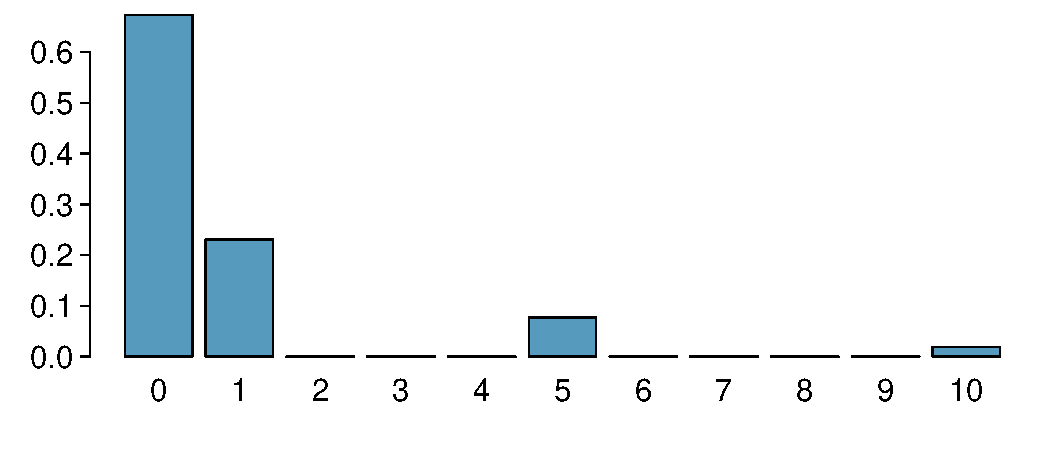
\includegraphics[width=0.8\textwidth]{\chp3@path/3-4_random_variables/figures/card_game/card_game}
\end{center}

\end{frame}

%%%%%%%%%%%%%%%%%%%%%%%%%%%%%%%%%%%%

%%%%%%%%%%%%%%%%%%%%%%%%%%%%%%%%%%%%

\section{Edfinity Quiz}

%%%%%%%%%%%%%%%%%%%%%%%%%%%%%%%%%%%%

% %%%%%%%%%%%%%%%%%%%%%%%%%%%%%%%%%%%%

% \subsection{Expectation}

% %%%%%%%%%%%%%%%%%%%%%%%%%%%%%%%%%%%%

% \begin{frame}
% \frametitle{Expectation}

% \begin{itemize}

% \item We are often interested in the average outcome of a random variable.

% \item We call this the \hl{expected value} (mean), and it is a weighted average of the possible outcomes
% \formula{\[\mu = E(X) = \sum_{i = 1}^k x_i ~ P(X = x_i)\]}

% \end{itemize}

% \end{frame}

% %%%%%%%%%%%%%%%%%%%%%%%%%%%%%%%%%%%%

% \begin{frame}
% \frametitle{Expected value of a discrete random variable}

% \dq{In a game of cards you win \$1 if you draw a heart, \$5 if you draw an ace (including the ace of hearts), \$10 if you draw the king of spades and nothing for any other card you draw. Write the probability model for your winnings, and calculate your expected winning.}

% \begin{center}
% \renewcommand{\arraystretch}{1.5}
% \begin{tabular}{l | c | c | c }
% Event		& $X$ 		& $P(X)$        		& $X ~ P(X)$ \\
% \hline
% Heart (not ace)	& $1$		& $\frac{12}{52}$	& $\frac{12}{52}$ \\
% Ace			& $5$		& $\frac{4}{52}$	& $\frac{20}{52}$ \\	
% King of spades	& $10$		& $\frac{1}{52}$	& $\frac{10}{52}$ \\	
% All else		& $0$		& $\frac{35}{52}$	& $0$ \\
% \hline
% Total			&			&		1		& $E(X) = \frac{42}{52} \approx 0.81$
% \end{tabular}

% \end{center}

% \end{frame}

% %%%%%%%%%%%%%%%%%%%%%%%%%%%%%%%%%%%%

% \subsection{Variability in random variables}

% %%%%%%%%%%%%%%%%%%%%%%%%%%%%%%%%%%%%

% \begin{frame}
% \frametitle{Variability}

% We are also often interested in the variability in the values of a random variable.

% \formula{
% \[ \sigma^2 = Var(X) = \sum_{i = 1}^k (x_i - E(X))^2 P(X = x_i) \]
% \[ \sigma = SD(X) = \sqrt{Var(X)} \]
% }

% \end{frame}

% %%%%%%%%%%%%%%%%%%%%%%%%%%%%%%%%%%%%

% \begin{frame}
% \frametitle{Variability of a discrete random variable}

% \dq{For the previous card game example, how much would you expect the winnings to vary from game to game?}

% \vspace{2mm}
% \only<2->{
% {\footnotesize
% \begin{center}
% \renewcommand{\arraystretch}{2}
% \begin{tabular}{c | c | c | l | p{4cm}}
% $X$ & $P(X)$         & $X ~ P(X)$      & \multicolumn{1}{c|}{$(X - E(X))^2$}  & \multicolumn{1}{c}{$P(X) ~ (X - E(X))^2$}  \\
% \hline
% 1 & $\frac{12}{52}$  & $1 \times \frac{12}{52} = \frac{12}{52}$ & $(1 - 0.81)^2 = 0.0361$ &  $\frac{12}{52} \times 0.0361 = 0.0083$ \\
% \hline
% 5 & $\frac{4}{52}$   & $5 \times \frac{4}{52} = \frac{20}{52}$ & $(5 - 0.81)^2 = 17.5561$  & $\frac{4}{52} \times 17.5561 = 1.3505$ \\
% \hline
% 10  & $\frac{1}{52}$ & $10 \times \frac{1}{52} = \frac{10}{52}$  & $(10 - 0.81)^2 = 84.4561$   & $\frac{1}{52} \times 84.0889 = 1.6242$ \\
% \hline
% 0 & $\frac{35}{52}$  & $0 \times \frac{35}{52} = 0$  & $(0 - 0.81)^2 = 0.6561$ & $\frac{35}{52} \times 0.6561 = 0.4416$ \\
% \hline
%   &       & $E(X) = 0.81$ & & \soln{\only<3->{$V(X) = 3.4246$}} \\
%  &       &                                                         & & \soln{\only<4>{$SD(X) = \sqrt{3.4246} = 1.85$}} \\
% \end{tabular}
% \end{center}
% }
% }
% \end{frame}

% %%%%%%%%%%%%%%%%%%%%%%%%%%%%%%%%%%%%

% \section{R Demonstration}

% %%%%%%%%%%%%%%%%%%%%%%%%%%%%%%%%%%%%

% %%%%%%%%%%%%%%%%%%%%%%%%%%%%%%%%%%%%

% \subsection{Linear combinations of random variables}

% %%%%%%%%%%%%%%%%%%%%%%%%%%%%%%%%%%%%

% \begin{frame}
% \frametitle{Linear combinations}

% \begin{itemize}

% \item A \hl{linear combination} of random variables $X$ and $Y$ is given by

% \[ aX + bY \]

% where $a$ and $b$ are some fixed numbers.

% \pause

% \item The average value of a linear combination of random variables is given by
% \formula{\[ E(aX + bY) = a \times E(X) + b \times E(Y) \]}

% \end{itemize}

% \end{frame}

% %%%%%%%%%%%%%%%%%%%%%%%%%%%%%%%%%%%%

% \begin{frame}
% \frametitle{Calculating the expectation of a linear combination}

% \dq{On average, a statistics homework has 20.3 problems and a physics homework has 5.4 problems. You take 5 minutes for each statistics problem and 25 minutes for each physics problem. On average, how much time should you expect to spend on homework every week?}

% \soln{
% \pause
% Let $S$ be the number of statistics problems and $P$ be the number of physics problems. 
% \begin{align*} 
% E(5S+25P) &= 5 \times E(S) + 25 \times E(P) \\
% &= 5 \times 20.3 + 25 \times 5.4 \\
% &= 101.5 + 135 \\
% &= 236.5~min = 3.94~hours
% \end{align*}
% }

% \end{frame}

% %%%%%%%%%%%%%%%%%%%%%%%%%%%%%%%%%%%%

% \subsection{Variability in linear combinations of random variables}

% %%%%%%%%%%%%%%%%%%%%%%%%%%%%%%%%%%%%

% \begin{frame}
% \frametitle{Linear combinations}

% \begin{itemize}

% \item The variability of a linear combination of two independent random variables is calculated as
% \formula{\[ V(aX + bY) = a^2 \times V(X) + b^2 \times V(Y) \]}

% \pause 

% \item The standard deviation of the linear combination is the square root of the variance.

% \end{itemize}

% \pause 
% \vfill

% \Note{If the random variables are not independent, the variance calculation gets a little more complicated and is beyond the scope of this course.}

% \end{frame}

% %%%%%%%%%%%%%%%%%%%%%%%%%%%%%%%%%%%%

% \begin{frame}
% \frametitle{Calculating the variance of a linear combination}

% \dq{The standard deviation of the number of statistics problems per homework is 2.3 problems, and it is 0.5 problems for physics homeworks. What is the standard deviation of the time you expect to spend on homework for the week? Assume that the number of problems on your statistics homework is independent of the number of problems on your physics homework.}

% \soln{
% \pause
% \begin{align*} 
% V(5S+25P) &= V(5S) + V(25P) \\
% &= 5^2 \times V(S) + 25^2 \times V(P) \\
% &= 25 \times 2.3^2 + 625 \times 0.5^2 \\
% &= 288.5
% \end{align*}
% \pause
% The standard deviation is $\sqrt{288.5} = 16.99~min = 0.28~hours$
% }

% \end{frame}

% %%%%%%%%%%%%%%%%%%%%%%%%%%%%%%%%%%%%

% % \section{Edfinity Quiz}

% %%%%%%%%%%%%%%%%%%%%%%%%%%%%%%%%%%%%



%%%%%%%%%%%%%%%%%%%%%%%%%%%%%%%%%%%%
% End document
%%%%%%%%%%%%%%%%%%%%%%%%%%%%%%%%%%%%

\end{document}